\section{DVI decoder}

\subsection{\texttt{dvi2rgb} module overview}
\begin{figure}
  \centering
  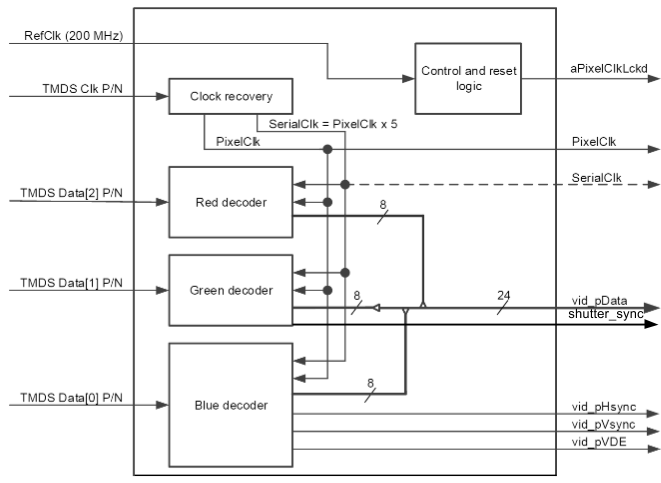
\includegraphics[width=1\textwidth]{./img/dvi2rgb.png}\par
  \caption{Block diagram of the DVI decoder \cite{dvi2rgb}.}
  \label{fig:dvi2rgb}
\end{figure}

The DVI decoder is connected via a \gls{hdmi} cable to the output of the DVI encoder on the sensor module board. It is important to note that the \gls{hdmi} port is connected directly to the \gls{fpga} and can be used to transmit anything provided the \gls{fpga} is configured correctly. The \gls{hdmi} ports have been carefully routed to carry four high-speed differential signals --- their controlled impedance makes them ideally suited to cope with the required bandwidth. As with the encoder, each channel is independent and so three identical decoders are instantiated, the output of which is concatenated to produce a 24-bit pixel bus accompanied by the standard video timing and synchronisation signals which are derived from the control data bits. In this proof-of-concept system the 8-bit pixel values from the OV7670 are tapped from the Blue channel on the receiver, a single control bit for the shutter synchronisation signal is tapped from the Green channel, and the Red channel remains unused.

\section{Clock recovery}
As the system is source-synchronous, the \gls{dvi} clock channel is used to drive the \gls{dvi} decoder logic on the receiver. The clock channel cannot be used directly, rather it contains a character-rate reference signal which is fed into a \gls{pll} to generate the pixel clock and serial clocks needed for the decoder logic to function. To generate these clocks an MMCME2\_ADV primitive, providing clock management functionality, is instantiated inside the \gls{dvi} decoder. Figure \ref{fig:clock_recovery} illustrates how the differential \gls{tmds} clock is fed into a differential input global clock buffer (\texttt{IBUFGDS}) connected to the input of the \gls{mmcm} primitive. The \gls{mmcm} contains a \gls{pll} clock multiplier which locks on to the reference clock and generates an output clock with a frequency five times higher. The output clock from the \gls{mmcm} is split and fed into two buffers. The first, a \texttt{BUFIO} primitive, provides the serial clock for the \texttt{ISERDESE2} primitives in the deserialisation logic. The second buffer is a \texttt{BUFR} primitive which has a frequency divider on it, which is used to divide the 5x serial clock back down and thus is how the pixel clock is generated. 

\begin{figure}
  \centering
  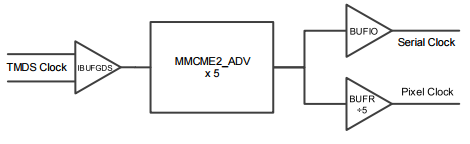
\includegraphics[width=1\textwidth]{./img/clock_recovery.png}
  \caption{Clock recovery overview \cite{dvi2rgb}.}
  \label{fig:clock_recovery}
\end{figure}

Inside the \gls{pll} a \gls{vco} is used is to generate an internal clock which can be varied by the feedback loop until it is locked to the reference clock \texttt{TMDS\_Clk}. The \gls{vco} operates at a frequency of \(FVCO = FIN * MULT_F\), meaning for an input \texttt{PixelClk} of \SI{12}{\mega\hertz} (as is the case with the OV7670), the \gls{vco} would oscillate at \SI{60}{\mega\hertz} due to the x5 multiplier. Unfortunately the \gls{vco} has a limited operating range between \SI{600}{\mega\hertz} and \SI{1200}{\mega\hertz}, to work with a \SI{12}{\mega\hertz} reference clock, the multiplier would need to be set to 50 to bring it up into the correct operating range, and then the output clock would need dividing by 10 to restore the 1:5 input / output ratio \cite{xilinx:ds187}.

Using the simple Python script in Listing \ref{lst:pll_calc} to naively search through the entire parameter space, no single set of PLL parameters will satisfy the full range of input frequencies while operating within the \gls{vco} limits. This means that the input frequency must be known prior to synthesis so the correct \gls{pll} parameters can be set. However, it is not uncommon for manufacturers to be conservative with their limits, and it happens that the \gls{vco} can operate far below the specified limits --- all of the tests performed were done with the gls{pll} parameters set for a \texttt{PixelClk} of \SI{148.5}{\mega\hertz}, despite the actual input being \SI{50}{\mega\hertz}. 

\begin{lstlisting}[caption={PLL parameter calculator script.}, label={lst:pll_calc}, language=Python]
"""A small script to calculate PLL parameters for target clocks.
This is easily the least efficient way to do it, but the search space
is pretty small so it's easier to just brute-force it. A parametric
solver would be better....

"""

CLK_IN1 = [25.175, 148.5]
TARGET = 5
TOLERANCE = 1   # +/- 1 Hz

DIVCLK_DIVIDE = xrange(1, 107)
CLKFBOUT_MULT = xrange(2, 65)
CLKOUT0_DIV = xrange(1, 129)
FVCOMIN = 600
FVCOMAX = 1200

print("{:<13} {:<13} {:<11}".format('DIVCLK_DIVIDE', 'CLKFBOUT_MULT', 'CLKOUT0_DIV'))

for divclk in DIVCLK_DIVIDE:
    for mult in CLKFBOUT_MULT:
        for div in CLKOUT0_DIV:
            for clk_in in CLK_IN1:
                fvco = clk_in * mult / divclk
                fout = fvco / div
                if fvco < FVCOMIN or fvco > FVCOMAX \
                  or fout < clk_in * TARGET - TOLERANCE or fout > clk_in * TARGET + TOLERANCE:
                    solution_found = False
                    break

                solution_found = True
            
            if solution_found: 
                print("{:<13} {:<13} {:<11}".format(divclk, mult, div))
\end{lstlisting}

\section{Deserialisation}

Much like the \texttt{rgb2dvi} module, deserialisation is done by chaining together two \texttt{ISERDESE2} primitives in a cascaded 1:10 DDR topology. Unlike the transmitter, the receiver requires an additional synchronisation step to re-align the three channels with the clock channel, as they may be out-of-phase by the time they reach the receiver. To do this a 32-tap delay line \texttt{IDELAYE2} primitive is inserted in front of each \texttt{ISERDESE2} primitives. Because transistors take a finite period of time to drive the line from low to high (\textit{rise-time}) or high to low (\textit{fall-time}), it is crucial that the signal is sampled at the correct time to avoid sampling the transition point. Figure \ref{fig:eye_diagram} shows how an eye opening forms when successive signals are repeatedly overlaid to form an eye diagram. As jitter increases, the lines become thicker and the signal is stable for less time. The basic premise is to increment the delay until we find the eye opening, which provides the best place to sample the signal. The \gls{tmds} encoder sends a large string of successive control tokens during the blanking period. As the value of the control tokens is fixed, we can keep adjusting the delay increments until we sample a value which matches the 10-bit control token we expect during the blanking period. Each tap only adds a \SI{78}{\pico\second} delay, which is only enough to shift between a bit or two. To shift between entire characters (10-bits) in order to find the character boundaries requires a much greater delay, which is done using the \textit{bitslip} control inside the \texttt{ISERDESE2} primitive. The \texttt{PhaseAlign} and \texttt{ChannelBond} modules control a state machine which sequences the delay increments to ensure all three channels are aligned at the start of each blanking period.

A critical issue occurs when the input \texttt{PixelClk} frequency is below \SI{40}{\mega\hertz}, which corresponds to the maximum \SI{78}{\pico\second} delay of the delay line. With the \SI{12}{\mega\hertz} pixel clock from the OV7670, the clock period is so long that it is possible to exhaust all of the delay taps without finding stable zone inside the eye. To rectify this, the incoming pixel clock must be boosted to above \SI{40}{\mega\hertz} by injecting artificial duplicate frames at the transmitter in order to allow the eye opening to be found correctly.

\begin{figure}
  \centering
  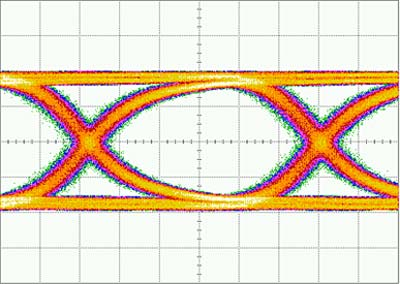
\includegraphics[width=1\textwidth]{./img/eye_diagram.jpg}
  \caption{\gls{serdes} eye diagram \cite{eye_diagram}.}
  \label{fig:eye_diagram}
\end{figure}

\section{TMDS decoding}

The decoding phase is far simpler than the encoding phase. A lookup table is used to see if the character matches any of the four known control tokens, and if so, sets the output accordingly. If the character is encoded data, the decoder XORs or XNORs each of the bits together to form the output.

\begin{lstlisting}[caption={TMDS decoding logic.}, label={lst:tmds_decode}, language=VHDL]
case (pDataInBnd) is
  --Control tokens decode straight to C0, C1 values
  when kCtlTkn0 =>
     pC0 <= '0';
     pC1 <= '0';
     pVde <= '0';
  when kCtlTkn1 =>
     pC0 <= '1';
     pC1 <= '0';
     pVde <= '0';               
  when kCtlTkn2 =>
     pC0 <= '0';
     pC1 <= '1';
     pVde <= '0';
  when kCtlTkn3 =>
     pC0 <= '1';
     pC1 <= '1';
     pVde <= '0';
  --If not control token, it's encoded data
  when others =>
     pVde <= '1'; 
     pDataIn(0) <= pDataIn8b(0);
     for iBit in 1 to 7 loop
        if (pDataInBnd(8) = '1') then
           pDataIn(iBit) <= pDataIn8b(iBit) xor pDataIn8b(iBit-1);
        else
           pDataIn(iBit) <= pDataIn8b(iBit) xnor pDataIn8b(iBit-1);
        end if;
     end loop;                           
end case;
\end{lstlisting}
